%Review of existing harmonic excitation.
%	Nonlinear Systems
%		Traditional Metrics (THD, IMD)
%		Minimisation of Nonlinear Distortion
%		Advent of "Nonlinear Niceness"
%	Timbre of nonlinear distortions (Martens and Marui type shit)
%	Uses of Harmonic Excitation
%	Harmonic Generation Methods
%		Static Nonlinearities
%		Bandwidth Extension (high frequency reconstruction)
%		Individual Harmonic Generation (SMC paper)
%		Psychoacoustic Enhancers

\chapter{Harmonic Excitation}

\section{Intro}
	\note{Harmonic excitation is of the chain. Look I wrote a paper about it \citep{Enderby2013Methods}.}

\section{Uses of Harmonic Excitation}

\section{Harmonic Generation Methods}
	\subsection{Static Nonlinearities}

	\subsection{Bandwidth Extension}
		\begin{figure}[h!]
			\centering
			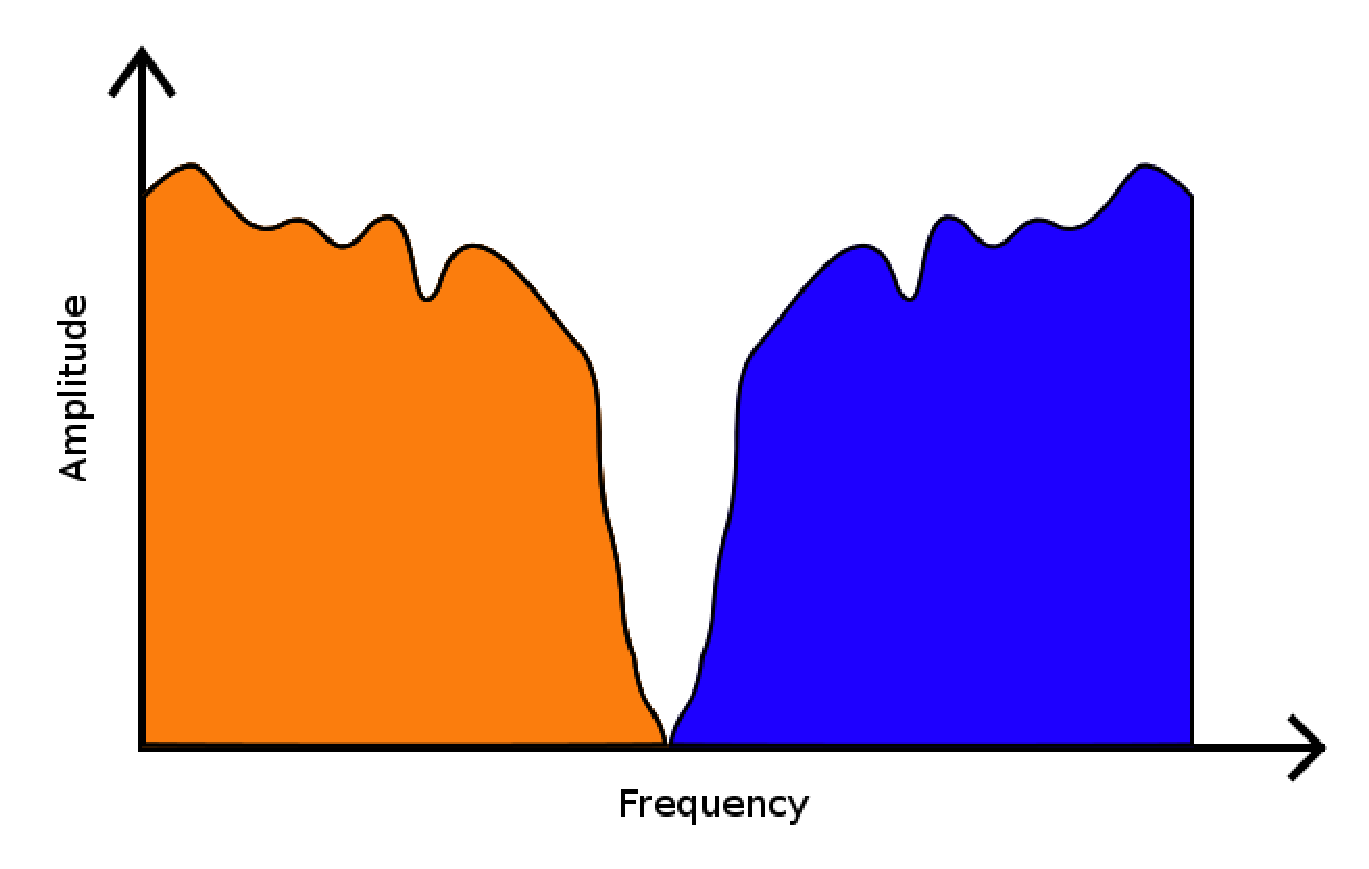
\includegraphics[width=0.5\textwidth]{Chapter3/Images/SpectralFolding.eps}
			\caption{Spectral Folding}
		\end{figure}

	\subsection{Individual Harmonic Generation}

	\subsection{Psychoacoustic Enhancers}
